%************************************************
\chapter{Elección del Algoritmo}
\label{ch:algorithm}
%************************************************

\citeauthor{yamada2003} \cite{yamada2003} proponen un método para analizar las
dependencias palabra-a-palabra mediante una estrategia \emph{bottom-up} -- de
abajo a arriba. -- Para ello se hace uso de la técnica de \ac{AA}
\acfi{SVM}. Sus experimentos se basan en árboles de dependencias creados a
partir del corpus \ac{PTB}, logrando una precisión superior al 90\% para
dependencias palabra-a-palabra. Aún siendo esta precisión inferior al
\nameref{sec:stateoftheart}, hay que tener en cuenta que este método no utiliza
información sobre la estructura de las frases.

El tipo de anotaciones usadas en este método pueden verse en la
\autoref{fig:deptree}. Esta forma de ilustrar las dependencias palabra-a-palabra
es más sencilla de entender para los anotadores que el usual estilo \ac{PTB} ---
\autoref{fig:strtree} --- El problema del estilo \ac{PTB} es que requiere que
los anotadores tengan un ámplio conocimiento de la teoría lingüística del
idioma, así como de la estructura de las frases, además del dominio específico
que trata el problema. Como ventaja adicional, la representación del árbol de
dependencias de la \autoref{fig:deptree} hace que la construcción de los datos
de entrenamiento sea menos ruidosa, al ser el proceso de anotación más simple.

\begin{figure}[h]
%\resizebox{1.3\textwidth}{!}{%
\tiny
\begin{tikzpicture}[every node/.style={align=center}]
  \tikzset{
    edge from parent/.style={
      draw,edge from parent
      path={(\tikzparentnode.south)-- +(0,-8pt)-| (\tikzchildnode)}
    },
    frontier/.style={distance from root=208pt}, % Align leaf nodes
    level 1+/.style={level distance=18pt} % Distance between levels
  }

   \Tree [.S
             [.NP Rolls-Royce\\NNP Motor\\NNP Cars\\NNPS Inc\\NNP ]
             [.VP said\\VBD
                [.SBAR [.none ]
                   [.S
                      [.NP it\\PRP ]
                      [. VP expects\\VBZ
                         [.S
                            [.NP its\\PRP\$ U.S\\NNP sales\\NNS ]
                            [.VP to\\TO
                               [.VP remain\\VB
                                  [.ADJP steady\\JJ ]
                                  [.PP at\\IN
                                     [.NP
                                        [.QP about\\IN 1200\\CD ]
                                        cars\\NNS
                                     ]
                                  ]
                               ]
                            ]
                         ]
                      ]
                   ]
                ]
             ]
         ]
\end{tikzpicture}
%}
\caption{Estructura en árbol de la frase ``Rolls-Royce Motor Cars Inc. said it
  expects its U.S. sales to remain steady at about 1,200 cars.''}
\label{fig:strtree}
\end{figure}

\begin{figure}[th]
  \scriptsize
  \begin{tikzpicture}[every node/.style={align=center},level distance=30pt]
    \tikzset{edge from parent/.append style={<-, >=latex,thick}}
   \Tree [.said\\VBD 
             [.Inc.\\NNP Rolls-Royce\\NNP Motor\\NNP Cars\\NNPS ]
             [.expects\\VBZ it\\PRP
                [.remain\\VB
                   [.sales\\NNS its\\PRP\$ U.S\\NNP ]
                   to\\TO
                   steady\\JJ 
                   [.at\\IN [.cars\\NNS [.about\\IN 1200\\CD ] ] ]
                ]
             ]
           ]
   \end{tikzpicture}
   \caption{Árbol de parseo de dependencias}
   \label{fig:deptree}
\end{figure}

En la estructura propuesta por \citeauthor{yamada2003} se realiza un análisis
estadístico de las dependencias de un idioma. Para lograr este análisis, el
algoritmo de aprendizaje escogido son \acp{SVM}, ya que son capaces de tratar
con espacios de características a gran escala. En los siguientes párrafos se
hará una breve intoducción a este algoritmo.

\section{Una introducción a las SVMs}
\label{subsec:svmintro}

\nocite{yaser2012} Los modelos lineales son muy poderosos, mediante
transformaciones lineales es posible incrementar en gran medida su capacidad
expresiva. Sin embargo, incrementar dicha capacidad tiene un precio, el sobre
ajuste y más tiempo de cómputo. \ac{SVM} usa un cojín de seguridad cuando separa
los datos. Este cojín logra que la \ac{SVM} sea más robusta al ruido, reduciendo
así el sobre ajuste. Además, \ac{SVM} es capaz de trabajar con la herramienta
conocida como \emph{kernel} --- la cual permite operar de forma eficiente con
transformaciones no lineales de gran dimensión ---. Estas dos características --
el cojín de seguridad y el \emph{kernel} -- hacen de la \ac{SVM} un modelo no
lineal muy robusto y potente con regularización automática. Las \ac{SVM} son muy
populares por su facilidad de uso y su buen rendimiento.

\ac{SVM} usa la estrategia del máximo márgen ideada por
\emph{Vapnik}. Supongamos $l$ datos de entrenamiento
$(\mathbf{x}_i,y_i), (1 \leq i \leq l)$, donde $\mathbf{x}_i$ es un vector de
características en un espacio de dimensionalidad $n$, $y_i$ es la etiqueta de la
clase $\{-1, +1\}$ de $\mathbf{x}$. Las \acp{SVM} encuentran un hiperplano
$\mathbf{w}\cdot \mathbf{x} + b = 0$ que separe correctamente los datos de
entrenamiento de forma que tengan margen máximo, es decir, con la máxima
distancia entre dos hiperplanos $\mathbf{w}\cdot \mathbf{x} + b \geq 1$ y
$\mathbf{w}\cdot \mathbf{x} + b \leq -1$, como se aprecia en la
\autoref{fg:svmexample}

\begin{figure}[h]
  \centering
  \missingfigure{SVM example}
  \caption{Ejemplo \ac{SVM}}
  \label{fg:svmexample}
\end{figure}

El uso de \ac{SVM} para el análisis estadístico de dependencias presenta
principalmente dos ventajas. La primera de ellas es un gran poder de
generalización en espacios de características de grandes dimensiones. Segunda,
gracias al \emph{kernel trick} es posible entrenar al modelo para que aprenda a
partir de la combinación de múltiples características.

Para poder trabajar con clasificaciones no lineales uno de los \emph{kernels}
posibles es el polinomial -- $(\mathbf{x}` \cdot \mathbf{x}`` + 1)^d$ -- Con
este \emph{kernel} se habilita la posibilidad de tener en cuenta combinaciones
de $d$ características sin incrementar demasiado el tiempo de cálculo. En el
problema que nos ocupa, esto se traduce en la capacidad de entrenar reglas de
dependencias usando varias características, como \ac{POS} \emph{tags}, las
palabras en sí y sus combinaciones.

%*****************************************
%*****************************************
%*****************************************
%*****************************************
%*****************************************
